\documentclass[border=6pt,tikz]{standalone}
\usepackage{tikz}
\usepackage{amsmath,amssymb}
\usetikzlibrary{arrows.meta,positioning,fit,backgrounds,calc,shapes.geometric,decorations.pathreplacing,patterns}
\definecolor{ink}{HTML}{1B2430}
\definecolor{muted}{HTML}{6B7785}
\definecolor{accent}{HTML}{2F6FB5}
\definecolor{accent2}{HTML}{C1611F}
\definecolor{good}{HTML}{2E7D5B}
\definecolor{soft}{HTML}{EDF2F7}
\definecolor{soft2}{HTML}{FBEDE2}
\definecolor{soft3}{HTML}{E6F0E9}
\tikzset{
  box/.style={draw=ink,line width=.7pt,rounded corners=2pt,fill=soft,inner sep=4pt,align=center,font=\sffamily\small},
  boxa/.style={box,fill=soft2},
  boxb/.style={box,fill=soft3},
  plain/.style={align=center,font=\sffamily\small,text=ink},
  tiny/.style={align=center,font=\sffamily\scriptsize,text=muted},
  ar/.style={-{Stealth[length=2.4mm]},draw=ink,line width=.7pt},
  arm/.style={-{Stealth[length=2.4mm]},draw=muted,line width=.6pt,dashed},
  nd/.style={circle,draw=ink,line width=.7pt,fill=white,minimum size=7mm,inner sep=0pt,font=\sffamily\scriptsize},
  ndf/.style={nd,fill=soft},
  ndt/.style={nd,fill=soft2},
}

\begin{document}
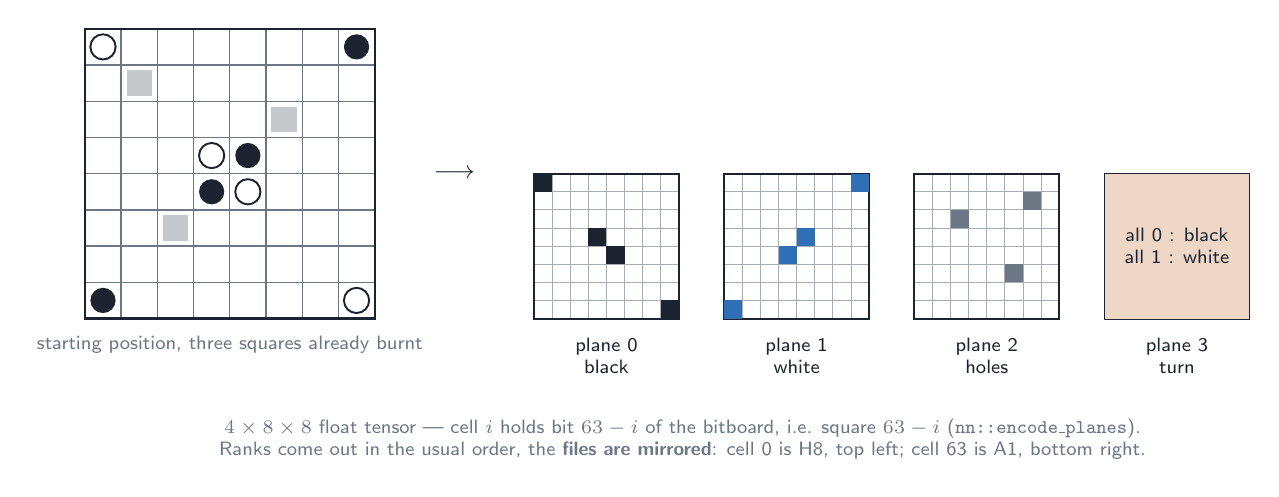
\begin{tikzpicture}[x=4.6mm,y=4.6mm]
  % ── the board ──
  \begin{scope}
    \draw[draw=muted,line width=.5pt,step=1] (0,0) grid (8,8);
    \draw[draw=ink,line width=.8pt] (0,0) rectangle (8,8);
    % black stones (X) : a1 h8 d4 e5  -> (col,row) 0-indexed from bottom-left
    \foreach \c/\r in {0/0,7/7,3/3,4/4} \fill[ink] (\c+.5,\r+.5) circle (1.6mm);
    % white stones (O) : h1 a8 e4 d5
    \foreach \c/\r in {7/0,0/7,4/3,3/4} {\draw[ink,line width=.7pt] (\c+.5,\r+.5) circle (1.6mm);}
    % holes
    \foreach \c/\r in {2/2,5/5,1/6} \fill[muted!40] (\c+.15,\r+.15) rectangle (\c+.85,\r+.85);
    \node[tiny,below=1mm] at (4,0) {starting position, three squares already burnt};
  \end{scope}

  \node[plain] at (10.2,4) {$\longrightarrow$};

  % ── the four planes ──
  \begin{scope}[shift={(12.4,0)},x=2.3mm,y=2.3mm]
    \foreach \i/\lbl/\col in {0/{plane 0\\black}/ink,1/{plane 1\\white}/accent,2/{plane 2\\holes}/muted,3/{plane 3\\turn}/accent2} {
      \begin{scope}[shift={(\i*10.5,0)}]
        \draw[draw=muted!60,line width=.3pt,step=1] (0,0) grid (8,8);
        \draw[draw=ink,line width=.7pt] (0,0) rectangle (8,8);
        \node[tiny,below=1.2mm,text=ink] at (4,0) {\lbl};
      \end{scope}
    }
    % The planes are the board with the FILES mirrored: plane column = 7 - file,
    % plane row = 7 - rank. So every board square (c, r) is drawn at (7-c, r).
    \begin{scope}\foreach \c/\r in {7/0,0/7,4/3,3/4} \fill[ink] (\c,\r) rectangle (\c+1,\r+1);\end{scope}
    \begin{scope}[shift={(10.5,0)}]\foreach \c/\r in {0/0,7/7,3/3,4/4} \fill[accent] (\c,\r) rectangle (\c+1,\r+1);\end{scope}
    \begin{scope}[shift={(21,0)}]\foreach \c/\r in {5/2,2/5,6/6} \fill[muted] (\c,\r) rectangle (\c+1,\r+1);\end{scope}

    \begin{scope}[shift={(31.5,0)}]\fill[accent2!25] (0,0) rectangle (8,8);\node[tiny,text=ink] at (4,4) {all 0 : black\\all 1 : white};\end{scope}
  \end{scope}

  \node[tiny,anchor=north] at (16.5,-2.5) {$4\times8\times8$ float tensor --- cell $i$ holds bit $63-i$ of the bitboard, i.e. square $63-i$ (\texttt{nn::encode\_planes}).\\
   Ranks come out in the usual order, the \textbf{files are mirrored}: cell 0 is H8, top left; cell 63 is A1, bottom right.};
\end{tikzpicture}
\end{document}
